% Generated by ic_study.analysis.v4_report_export from the v4 report with
% manifest SHA-256 6608b3960eb73011caca97870a4ffd3dbfbcd4c2df09bbbcb576c1c9452cf981.
% Edited during the journal revision (agent S, 2026-10-13): captions, headers and
% categorical cells in plain English; every number keeps its \resultnum binding.
\begin{figure*}[tp]
\centering
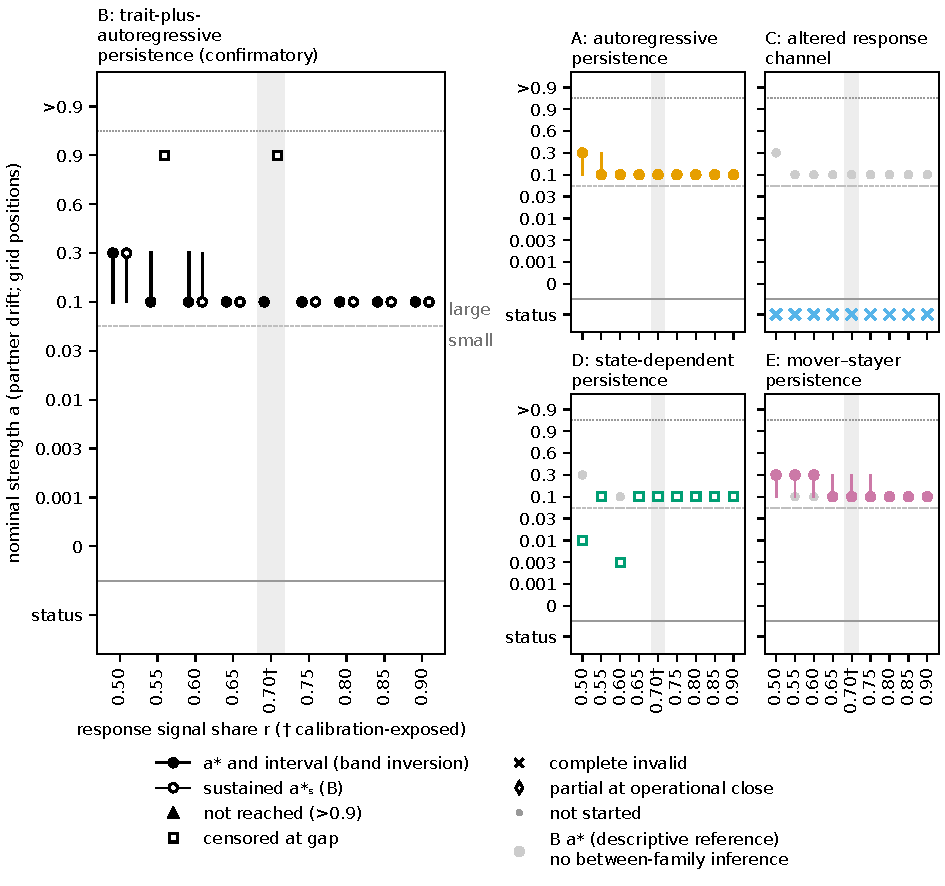
\includegraphics[width=\textwidth,height=175mm,keepaspectratio]{generated/F1_a_star_by_family.pdf}
\caption{Boundaries by persistence model, in the display of the rule-assembled record: first boundary $a^*(r)$ against B (trait plus autoregressive persistence) and against A (autoregressive), C (autoregressive with an altered response channel), D (state-dependent) and E (mover--stayer persistence). Horizontal axis: signal share $r$; vertical axis: influence strength $a$ at the positions of the grid (equal spacing does not mean equal increments; nothing is interpolated). Filled circles: $a^*$, with bars for its interval by inclusive inversion of the per-$r$ band; open circles: the sustained boundary $a_s^*$ of B. Triangles: not reached on the complete grid. Open squares mark a boundary censored at a gap; drawn on the top row, they mean censored at the gap at $a=0.90$, not a boundary at 0.90. The strip below each panel marks units without a valid curve (all nine C units). Gray B markers in the panels of the other models repeat the B boundaries as a visual reference only; no comparison across models is made. Bands are simultaneous over the strengths of one $r$ only. \dag\ $r=0.70$, examined during calibration.}\label{fig:v4-F1}
\end{figure*}
